\documentclass[12pt,a4paper,twoside,openright,titlepage,final]{article}
\usepackage{fontspec}
\usepackage{amsmath}
\usepackage{amsfonts}
\usepackage{amssymb}
\usepackage{makeidx}
\usepackage{graphicx}
\usepackage[hidelinks,unicode=true]{hyperref}
\usepackage[spanish,es-nodecimaldot,es-lcroman,es-tabla,es-noshorthands]{babel}
\usepackage[left=3cm,right=2cm, bottom=4cm]{geometry}
\usepackage{natbib}
\usepackage{microtype}
\usepackage{ifdraft}
\usepackage{verbatim}
\usepackage[obeyDraft]{todonotes}
\ifdraft{
	\usepackage{draftwatermark}
	\SetWatermarkText{BORRADOR}
	\SetWatermarkScale{0.7}
	\SetWatermarkColor{red}
}{}
\usepackage{booktabs}
\usepackage{longtable}
\usepackage{calc}
\usepackage{array}
\usepackage{caption}
\usepackage{subfigure}
\usepackage{footnote}
\usepackage{url}
\usepackage{tikz}
\tikzset{
  treenode/.style = {shape=rectangle, rounded corners,
                     draw, align=center,
                     top color=white, bottom color=blue!20},
  root/.style     = {treenode, font=\Large, bottom color=red!30},
  env/.style      = {treenode, font=\ttfamily\normalsize},
  dummy/.style    = {circle,draw}
}

\setsansfont[Ligatures=TeX]{texgyreadventor}
\setmainfont[Ligatures=TeX]{texgyrepagella}

%*******************************************************
%                 NO MODIFICAR
\newcommand*{\FSfont}[1]{%
  \fontencoding{T1}\fontfamily{#1}\selectfont}

\newlength{\tpheight}\setlength{\tpheight}{0.9\textheight}
\newlength{\txtheight}\setlength{\txtheight}{0.9\tpheight}
\newlength{\tpwidth}\setlength{\tpwidth}{0.9\textwidth}
\newlength{\txtwidth}\setlength{\txtwidth}{0.9\tpwidth}
\newlength{\drop}
%*******************************************************

% Crea una portada con los siguientes parámetros
%
% #1 : Título 
% #2 : Subtítulo
% #3 : Subsubtítulo
% #4 : Autor(es)
% #5 : Lugar
%

\newcommand*{\portada}[5]{
\begin{titlepage}
\begingroup
\vspace*{1cm}
\drop = 0.2\txtheight
\centering
\vfill
{\Huge \scshape #1}\\[\baselineskip]
{\Large \textbf{#2}}\\[\baselineskip]
{\Large \scshape #3}\\[\baselineskip]
\vspace*{0.3cm}
{\large \textit{#4}}\\[0.5\drop]

\includegraphics[scale=0.35]{./imagenes/logoURJC.jpg}
\vspace*{1.5cm}

{\large \scshape #5, \today} \par
\begin{center}
\end{center}
\vfill\null
\endgroup
\end{titlepage}
}
 %*****************************************************
 


\author{José Ignacio Escribano}

\title{Caso práctico II}

\setlength{\parindent}{0pt}

\begin{document}

\pagenumbering{alph}
\setcounter{page}{1}

\portada{Caso Práctico II}{Modelización y tratamiento de la incertidumbre}{Probabilidades y variables aleatorias}{José Ignacio Escribano}{Móstoles}

\listoffigures
\thispagestyle{empty}
\newpage

\tableofcontents
\thispagestyle{empty}
\newpage


\pagenumbering{arabic}
\setcounter{page}{1}

\section{Introducción}


\section{Resolución del caso práctico}



\subsection{Tarea VI}

El beneficio de cada inversión viene dado por la diferencia entre los beneficios netos y la inversión (1 millón de euros). Así, por tanto, si se pierde todo lo invertido tenemos que el beneficio es -1 (los beneficios netos son cero y la inversión 1); cuando no se obtiene beneficio neto ni se pierde la inversión tenemos que los beneficios son 0.\\

Si denotamos con $X_i$ al beneficio neto obtenido en la inversión $i$ con $i = 1,2,3$, tenemos que las funciones de masa vienen dadas de la siguiente forma:

\begin{equation*}
f(X_1 = x) = \begin{cases}
0.1, & \text{si } x = 5 \\
0.3, & \text{si } x = 1 \\
0.6, & \text{si } x = -1
\end{cases}
\end{equation*}

\begin{equation*}
f(X_2 = x) = \begin{cases}
0.2, & \text{si } x = 3 \\
0.4, & \text{si } x = 1 \\
0.4, & \text{si } x = -1
\end{cases}
\end{equation*}

\begin{equation*}
f(X_3 = x) = \begin{cases}
0.1, & \text{si } x = 6 \\
0.7, & \text{si } x = 0 \\
0.2, & \text{si } x = -3
\end{cases}
\end{equation*}

En la Figura~\ref{fig:funciones_masa_inversiones} se pueden ver las funciones de masa de las tres inversiones.\\ 

\begin{figure}[tbph!]
\centering
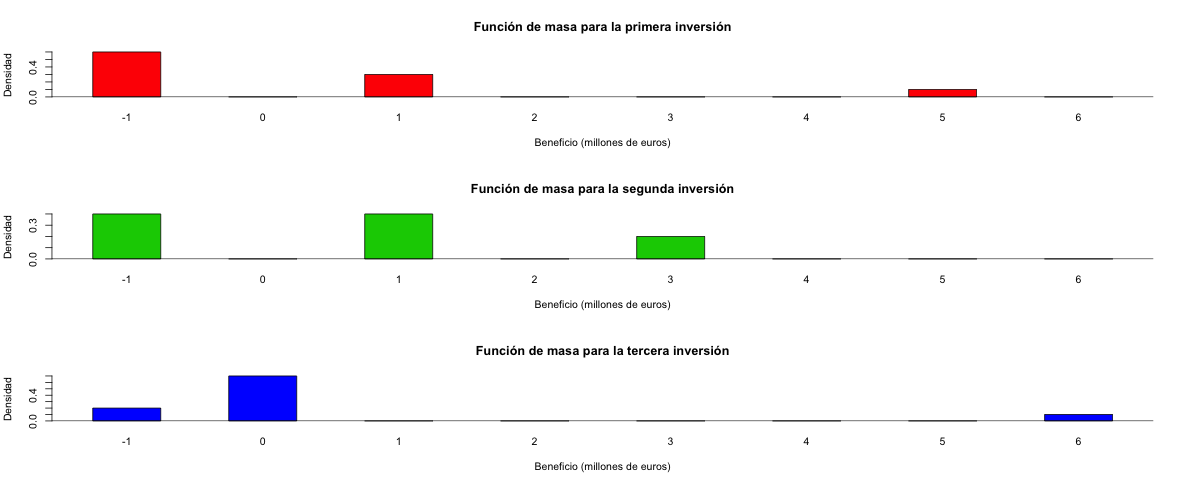
\includegraphics[width=0.9\linewidth]{imagenes/funciones_masa_inversiones}
\caption{Funciones de masa de las inversiones}
\label{fig:funciones_masa_inversiones}
\end{figure}

Calculamos la media y la varianza del beneficio de cada inversión.

\begin{align*}
E[X_1] & = \sum_{i \in \Omega_1} i\cdot f(X_1 = i) \\ & = 5 \cdot 0.1 + 1 \cdot 0.3 - 1 \cdot 0.6 \\ & = 0.2
\end{align*}

\begin{align*}
Var[X_1] & = \sum_{i \in \Omega_1} f(X_1 = i) (x_i - E[X_1])^2 \\ & = 0.1(5 - 0.2)^2 + 0.3(1-0.2)^2 + 0.6(-1 - 0.2)^2 \\ & = 3.36
\end{align*}

donde $\Omega_1 = \{-1, 1, 5\}$ es el soporte de la variable $X_1$.\\

De igual forma, se obtiene que 

\begin{align*}
E[X_2] & = 0.6 \\
Var[X_2] & = 2.24
\end{align*}

\begin{align*}
E[X_3] & = 0.4 \\
Var[X_3] & = 3.64
\end{align*}

con $\Omega_2 = \{-1, 1, 3\}$ y $\Omega_3 = \{-1, 0, 6\}$, los soportes de las variables $X_2$ y $X_3$, respectivamente.\\

Para ver la inversión más segura, calculamos la probabilidad de obtener beneficios, es decir, $P(X_i > 0)$ con $i = 1,2,3$. Así, tenemos que\\

\begin{align*}
P(X_1 > 0) & = 1 - P(X_1 \leq 0) \\ & = 1 - P(X_1 = -1) \\ & = 1 - 0.6 \\ & = 0.4
\end{align*}

\begin{align*}
P(X_2 > 0) & = 1 - P(X_2 \leq 0) \\ & = 1 - P(X_2 = -1) \\ & = 1 - 0.4 \\ & = 0.6
\end{align*}

\begin{align*}
P(X_3 > 0) & = 1 - P(X_3 \leq 0) \\ & = 1 - (P(X_3 = -1) + P(X_3 = 0)) \\ & = 1 - 0.7 - 0.2 \\ & = 0.1
\end{align*}

Vemos que la opción más segura para obtener algún beneficio es la segunda, ya que hay 60\% de probabilidades de ganar algo de dinero con esta inversión.\\

Para ver la inversión más arriesgada, calculamos la probabilidad de no perder dinero, es decir, $P(X_i \geq 0)$,

\begin{align*}
P(X_1 \geq 0) & = 1 - P(X_0 < 0) \\ & = 1 - P(X_1 = -1) \\ & = 1 - 0.6 \\ & = 0.4
\end{align*}

\begin{align*}
P(X_2 \geq 0) & = 1 - P(X_2 < 0) \\ & = 1 - P(X_2 = -1) \\ & = 1 - 0.4 \\ & = 0.6
\end{align*}

\begin{align*}
P(X_3 \geq 0) & = 1 - P(X_3 < 0) \\ & = 1 - P(X_3 = -1) \\ & = 1 - 0.2 \\ & = 0.8 
\end{align*}

La opción más arriesgada es la tercera, donde hay más probabilidades de no perder dinero, pero hay un 70\% de no ganar nada, aunque en caso de ganar, ganaremos la mayor cantidad de dinero de todas las inversiones, 6 millones de euros.\\

 

\subsection{Tarea V}



\subsection{Tarea VI}


\subsection{Tarea VII}

\section{Conclusiones}
   

\newpage

\section{Código R}

\verbatiminput{../caso_ii2.0.R}


\end{document} 